\documentclass[letterpaper]{article}
\usepackage[plots]{settings}

\begin{document}
\begin{notes}{Part 5: Geometry and Camera Models}

\NoteChapter{From the Object to the Digital Image}

A digital image is the end of a long chain. Light bounces off the scene, a lens focuses it, a sensor turns it into numbers, a processor turns those numbers into an image, and a screen turns the image back into light. The figure shows the whole chain for a digital camera; the sections below go through it step by step.

\begin{figure}[H]
\centering
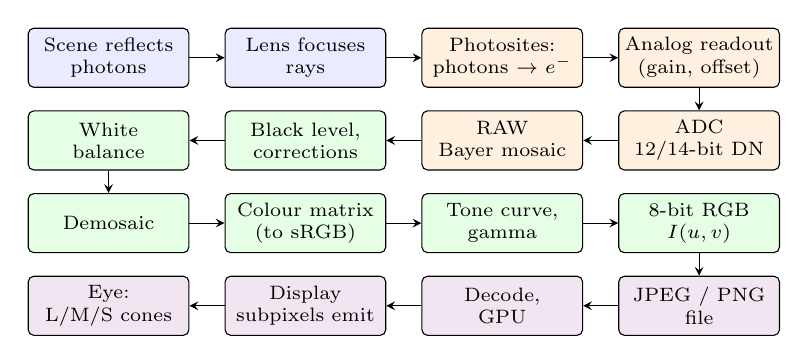
\begin{tikzpicture}[
    x=2.5cm, y=-1.05cm, >=stealth,
    box/.style={draw, rounded corners=2pt, font=\scriptsize, align=center,
                text width=1.9cm, minimum height=0.75cm, inner sep=2pt},
    optics/.style={box, fill=blue!8},
    sensor/.style={box, fill=orange!12},
    isp/.style={box, fill=green!10},
    output/.style={box, fill=violet!10}]
  % row 1: left to right
  \node[optics] (a1) at (0,0) {Scene reflects\\photons};
  \node[optics] (a2) at (1,0) {Lens focuses\\rays};
  \node[sensor] (a3) at (2,0) {Photosites:\\photons $\to e^-$};
  \node[sensor] (a4) at (3,0) {Analog readout\\(gain, offset)};
  % row 2: right to left
  \node[sensor] (b4) at (3,1) {ADC\\12/14-bit DN};
  \node[sensor] (b3) at (2,1) {RAW\\Bayer mosaic};
  \node[isp]    (b2) at (1,1) {Black level,\\corrections};
  \node[isp]    (b1) at (0,1) {White\\balance};
  % row 3: left to right
  \node[isp]    (c1) at (0,2) {Demosaic};
  \node[isp]    (c2) at (1,2) {Colour matrix\\(to sRGB)};
  \node[isp]    (c3) at (2,2) {Tone curve,\\gamma};
  \node[isp]    (c4) at (3,2) {8-bit RGB\\$I(u,v)$};
  % row 4: right to left
  \node[output] (d4) at (3,3) {JPEG / PNG\\file};
  \node[output] (d3) at (2,3) {Decode,\\GPU};
  \node[output] (d2) at (1,3) {Display\\subpixels emit};
  \node[output] (d1) at (0,3) {Eye:\\L/M/S cones};
  \draw[->] (a1)--(a2); \draw[->] (a2)--(a3); \draw[->] (a3)--(a4); \draw[->] (a4)--(b4);
  \draw[->] (b4)--(b3); \draw[->] (b3)--(b2); \draw[->] (b2)--(b1); \draw[->] (b1)--(c1);
  \draw[->] (c1)--(c2); \draw[->] (c2)--(c3); \draw[->] (c3)--(c4); \draw[->] (c4)--(d4);
  \draw[->] (d4)--(d3); \draw[->] (d3)--(d2); \draw[->] (d2)--(d1);
\end{tikzpicture}
\caption{The imaging chain. Blue: optics; orange: sensor and digitisation; green: image signal processor; violet: storage and display.}
\end{figure}

\NoteSection{Scene and Optics}

\begin{enumerate}[series=steps]
    \item \textbf{Light leaves the scene as photons.} A light source (the Sun, a lamp) lights the scene. Objects absorb some of that light and reflect the rest, and some of the reflected photons reach the camera. Different objects reflect different amounts and colours of light:
    \begin{itemize}[noitemsep]
        \item a white object reflects most visible light;
        \item a black object reflects very little;
        \item a red object reflects mostly red light.
    \end{itemize}

    \begin{figure}[H]
      \centering
      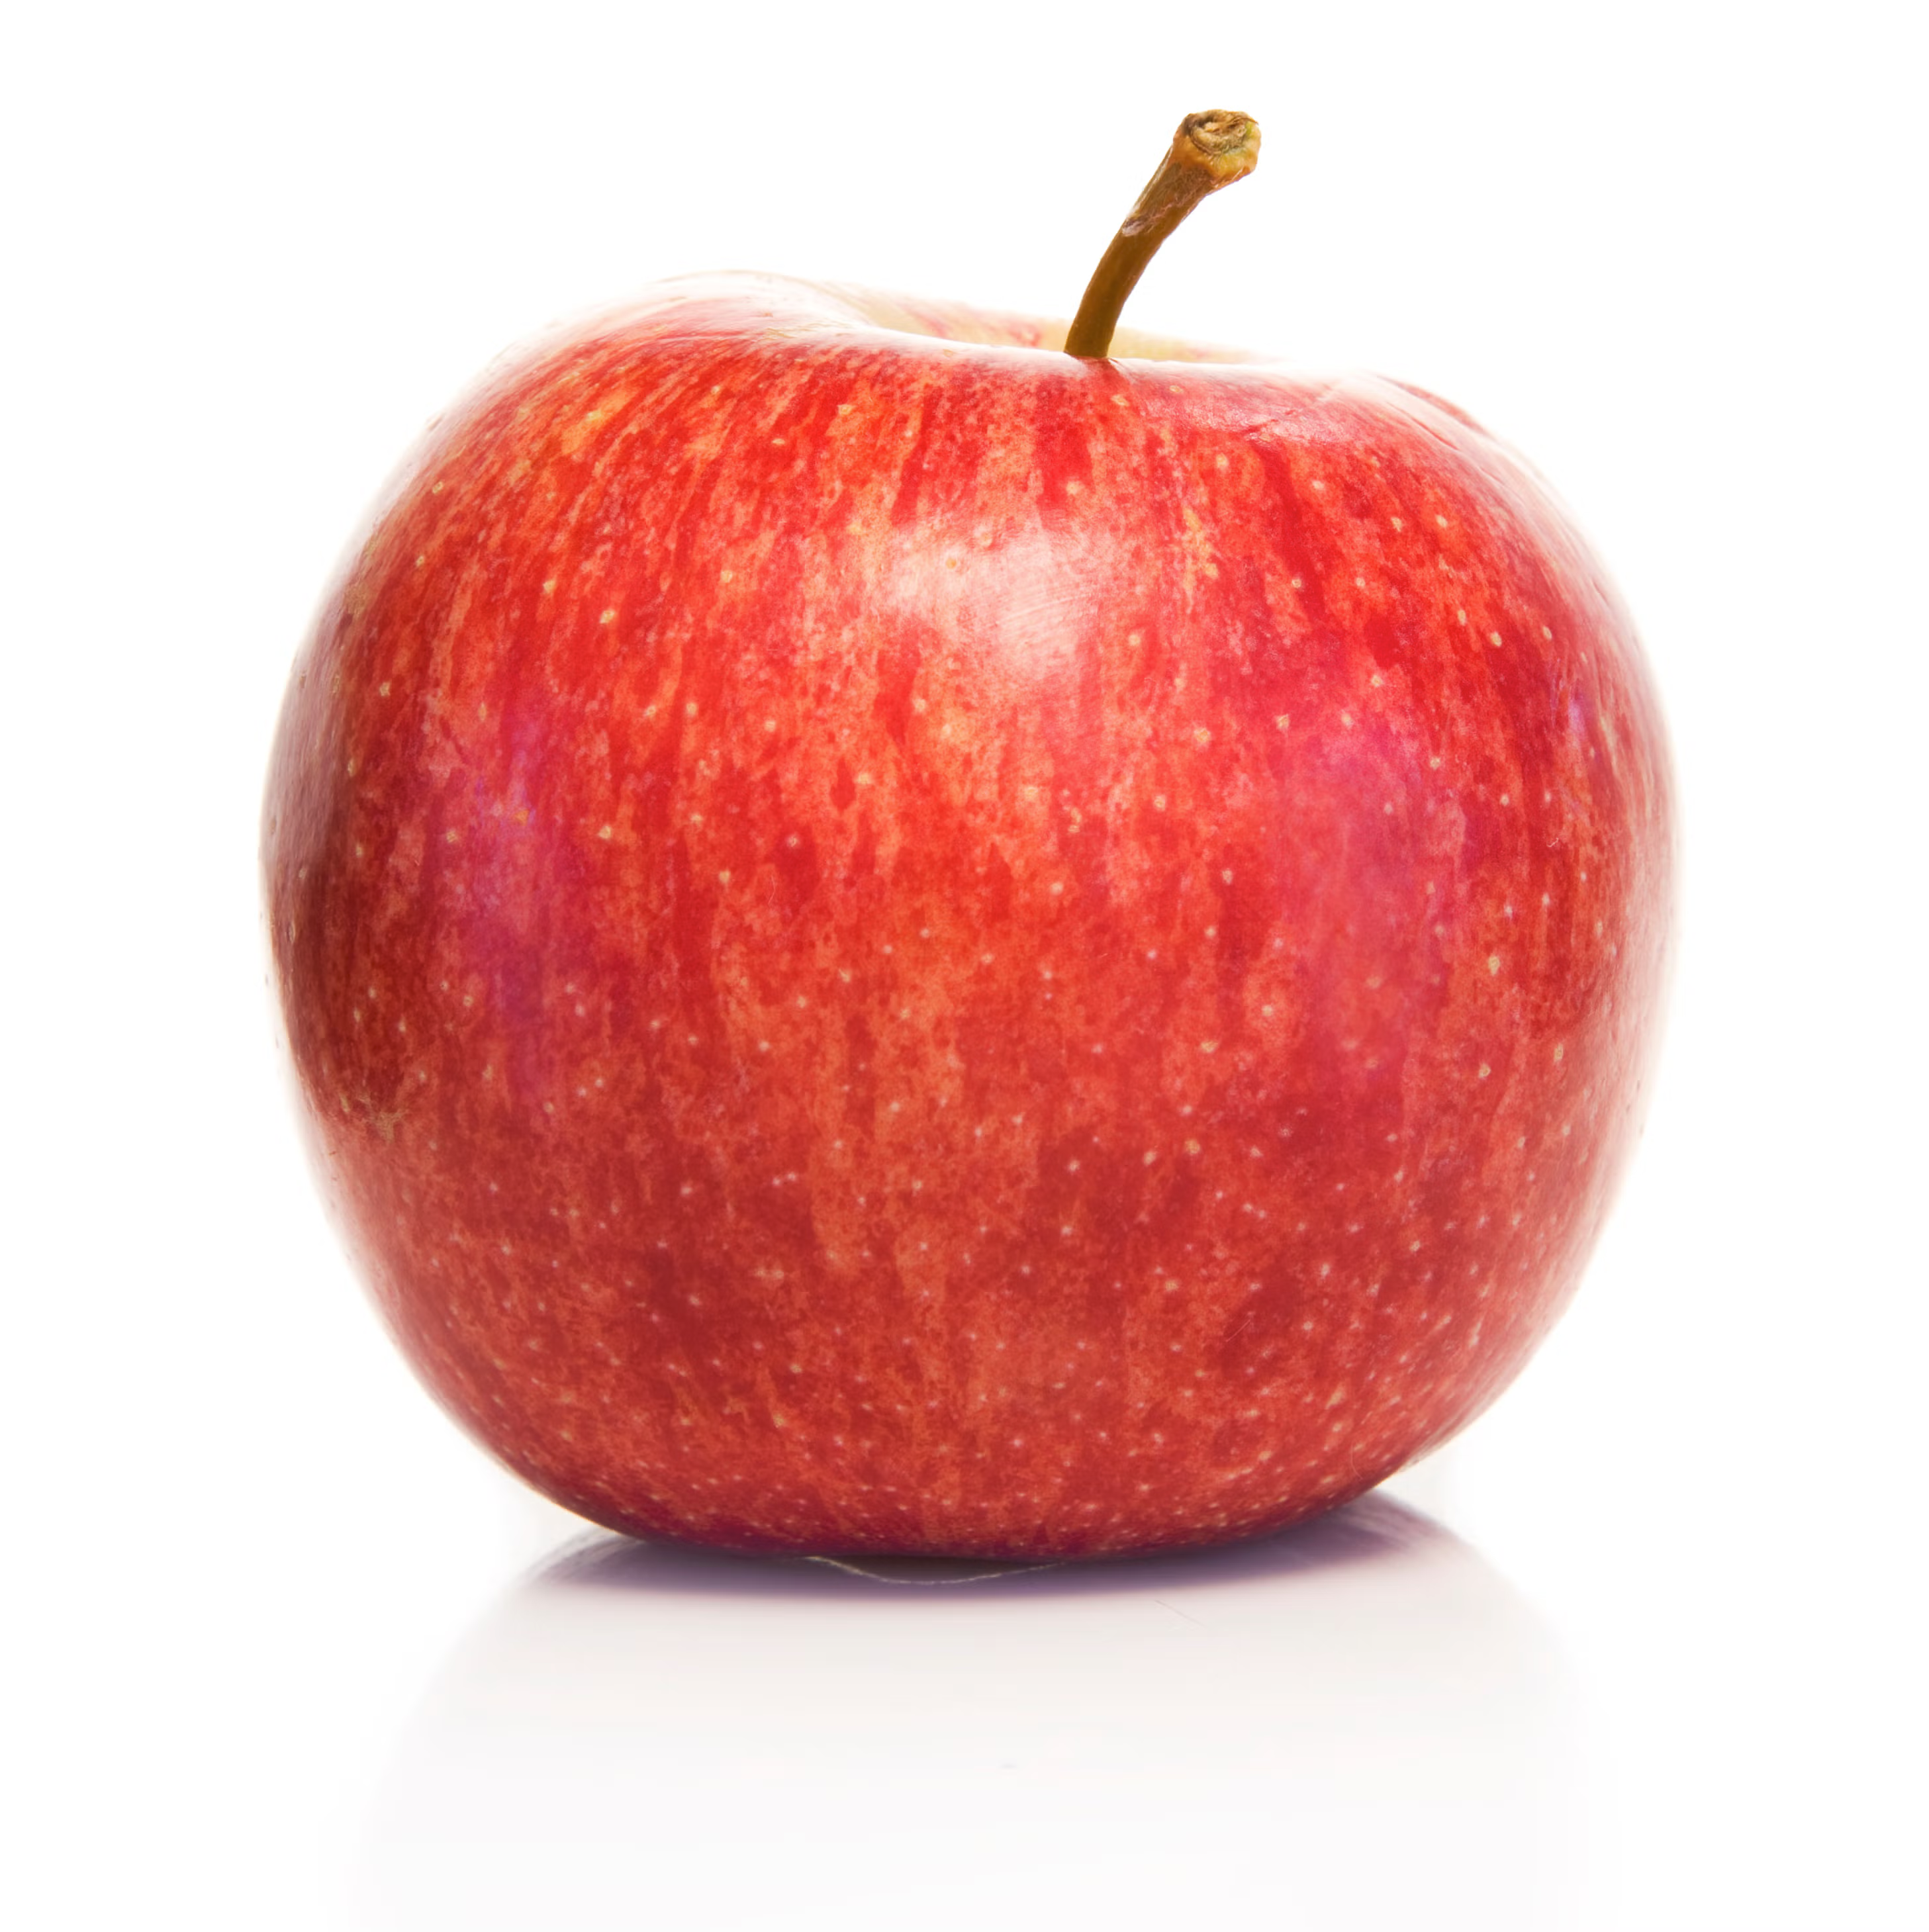
\includegraphics[width=0.35\linewidth]{images/part5/apple.png}
      \caption{An apple.}
    \end{figure}

    The spectrum reaching the camera is the product of the illuminant's spectrum and the surface's reflectance - which is why the same object looks different under sunlight and tungsten, and why white balance (step~\ref{step:wb}) is needed.
    \item \textbf{The lens focuses the rays.} Every scene point radiates in all directions, so a bare sensor would receive light from every point at every photosite and record only a uniform blur. The lens bends the rays so that photons from one 3-D scene point converge on one sensor location - this is what turns a 3-D scene into a 2-D image. The pinhole model of the next chapter idealises the aperture as a single point and asks only \emph{where} each point lands.
    \begin{figure}[H]
      \centering
      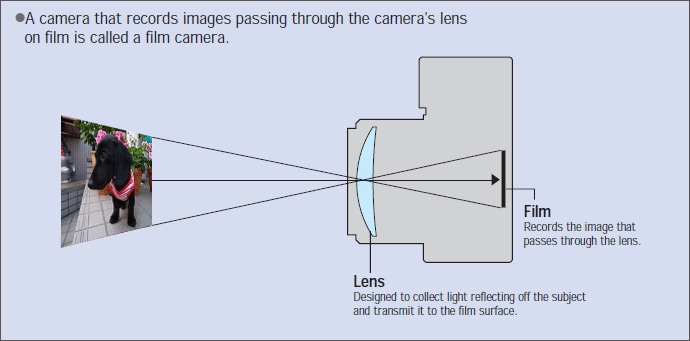
\includegraphics[width=0.8\linewidth]{images/part5/camera-lens.png}
      \caption{The lens focuses light from the scene onto the sensor.}
    \end{figure}
\end{enumerate}

\NoteSection{Sensor and Colour Filter Array}

\begin{enumerate}[resume=steps]
    \item\label{step:sensor} \textbf{Photons hit the sensor.} Behind the lens sits a silicon sensor (almost always CMOS today) - a grid of millions of photosensitive \emph{photosites}, from roughly $0.6\,\mu$m pitch in phones to about $6\,\mu$m in full-frame cameras. Each photosite integrates the light arriving at its location during the exposure; this is where the physical world becomes an electrical measurement.
    
    \begin{figure}[H]
      \centering
      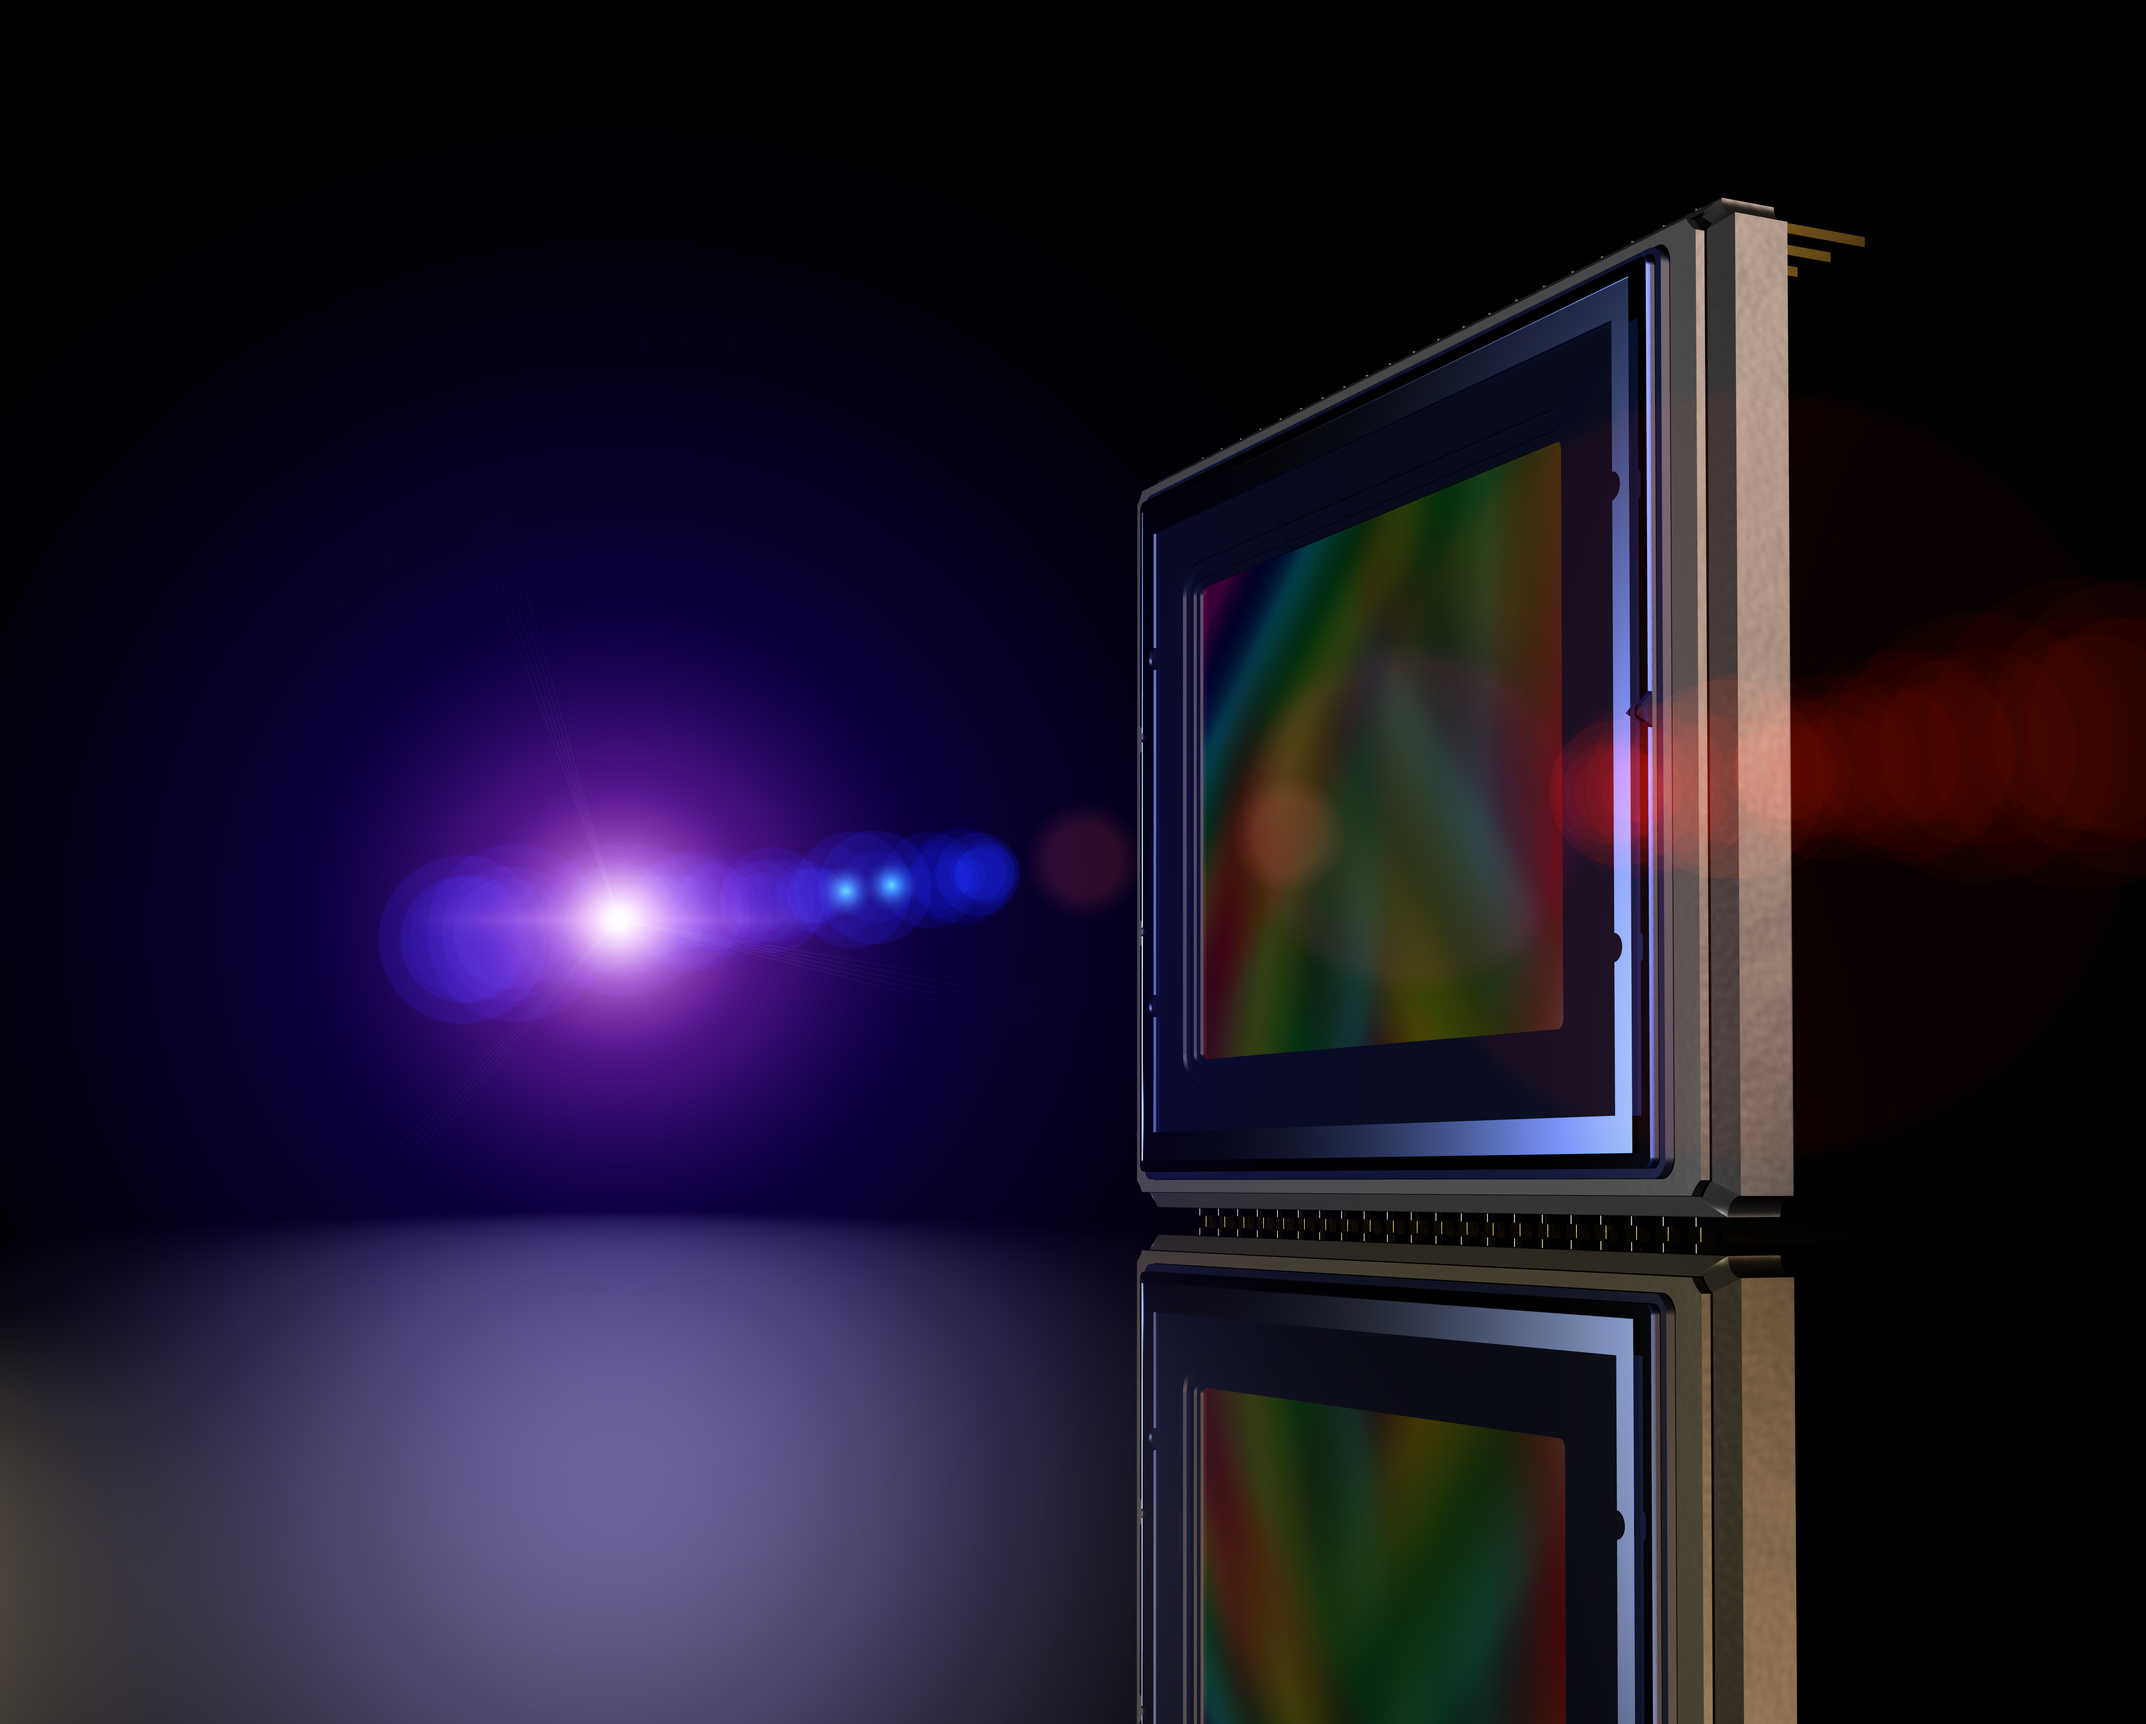
\includegraphics[width=0.4\linewidth]{images/part5/sensor.png}
      \caption{The Sony IMX430 CMOS sensor.}
    \end{figure}


    \item \textbf{Photons generate electrons.} Via the photoelectric effect, an absorbed photon frees an electron, and the photosite accumulates charge over the exposure:
    $$\text{more photons}\;\to\;\text{more electrons}\;\to\;\text{larger signal}.$$
    With a quantum efficiency of about $60\%$, a dark patch delivering $50$ photons yields about $30\,e^-$, while a bright patch delivering $30{,}000$ photons yields about $18{,}000\,e^-$. The result is not yet an image - only millions of charge packets, one per photosite. The section on CMOS sensors below looks at how the photosite actually does this.
    \item \textbf{Colour is sampled by a filter array.} A bare photosite measures \emph{how much} light arrives, not its colour - it cannot report ``37\% red, 42\% green, 21\% blue''. A \textbf{colour filter array} (CFA) over the sensor makes each photosite respond predominantly to one band. The usual layout is the \textbf{Bayer pattern}, with twice as many green sites as red or blue because green carries most of the luminance the eye is sensitive to:
    \begin{center}
    \begin{tabular}{cccc}
        G & R & G & R \\
        B & G & B & G \\
        G & R & G & R \\
        B & G & B & G
    \end{tabular}
    \end{center}
    Each location therefore measures one colour, and the other two are simply missing. Raw sensor data is a \emph{mosaic}, not an RGB image.
\end{enumerate}

\NoteSection{Readout and Digitisation}

\begin{enumerate}[resume=steps]
    \item \textbf{The analog signal is read out.} Each photosite's charge is converted to a voltage and read off the sensor row by row. Along the way the signal is
    \begin{itemize}[noitemsep]
        \item amplified by the analog gain (the camera's ISO setting);
        \item shifted by a black-level offset, so that noise below zero is not clipped;
        \item corrupted by read noise and other noise sources (see Part 2).
    \end{itemize}
    All of these are still analog quantities.
    \item\label{step:adc} \textbf{The ADC quantises the signal.} An \textbf{analog-to-digital converter} maps each voltage to an integer \textbf{digital number} (DN). A 12-bit ADC gives $2^{12}=4096$ levels, $\mathrm{DN}\in\{0,\ldots,4095\}$; a 14-bit ADC gives $16{,}384$. For example, with a 12-bit ADC,
    $$\text{small signal}\to 217,\qquad \text{medium}\to 1832,\qquad \text{large}\to 3901.$$
    From here on the data is digital.
    \item \textbf{The result is RAW data.} A 2-D array of 12- or 14-bit DNs, one per photosite, still in the Bayer mosaic and in the sensor's own colour response. The top-left corner of a RAW frame might read
    \begin{center}
    \begin{tabular}{cccc}
        \scriptsize G & \scriptsize R & \scriptsize G & \scriptsize R \\[-3pt]
        1832 & 924 & 2103 & 451 \\
        \scriptsize B & \scriptsize G & \scriptsize B & \scriptsize G \\[-3pt]
        388 & 1790 & 402 & 2011
    \end{tabular}
    \end{center}
    where the letters are \emph{not} stored - they are implied by the known CFA layout. Each position holds a single number. This is what a RAW file stores: sensor \emph{measurements}, not a displayable image.
\end{enumerate}

\NoteSection{Inside a CMOS Image Sensor}

Steps~\ref{step:sensor}-\ref{step:adc} happen inside the sensor. This section looks at how. The noise sources involved (read noise, $kTC$ noise, dark current, full well and dynamic range, column FPN) are covered in Part 2 and not repeated here.

\NoteSubsection{The Photodiode}

\textbf{Charge generation.} Each photosite is a reverse-biased \textbf{p-n junction photodiode}. A photon with energy above silicon's band gap ($E_g = 1.12$\,eV) can lift an electron into the conduction band, creating an electron-hole pair. The electric field of the depletion region separates the pair, and the electron is held in the potential well of the photodiode until readout. Silicon therefore responds up to
$$\lambda_{\max} = \frac{hc}{E_g} \approx \frac{1.24\,\mu\text{m}\cdot\text{eV}}{1.12\,\text{eV}} \approx 1.1\,\mu\text{m},$$
which is why silicon sensors see near-infrared and why visible cameras carry an \textbf{IR-cut filter}.

\textbf{Absorption depth depends on wavelength.} Blue light is absorbed within about $0.5\,\mu$m of the surface, red within a few $\mu$m, and near-infrared penetrates $10\,\mu$m or more. Photodiode depth therefore sets the spectral response, and long-wavelength photons absorbed deep in the substrate can diffuse into a neighbouring pixel (\emph{crosstalk}).

\textbf{Key figures of merit.}
\begin{itemize}[noitemsep]
    \item \textbf{Quantum efficiency} (QE): fraction of incident photons that produce a collected electron; about $50$-$80\%$ at the peak for modern sensors.
    \item \textbf{Full-well capacity}: the most charge a pixel can hold before it saturates. It scales roughly with pixel area, from a few thousand $e^-$ in small phone pixels to $50{,}000$-$100{,}000\,e^-$ in large ones.
    \item \textbf{Fill factor}: fraction of the pixel area that is light-sensitive. Transistors and wiring take up the rest.
    \item \textbf{Conversion gain}: output voltage per electron at the sense node, $\mathrm{CG} = q/C_{\mathrm{FD}}$, typically tens of $\mu$V$/e^-$. A smaller sense capacitance means higher gain and lower input-referred noise.
\end{itemize}

\textbf{Microlenses.} A tiny lens above each pixel focuses light away from the insensitive areas and onto the photodiode, raising the effective fill factor. Toward the edge of the sensor, light arrives at an oblique \emph{chief ray angle}, so the microlenses are shifted slightly toward the centre to compensate. Without that shift, the edges of the image would be darker (a form of vignetting).

\NoteSubsection{Pixel Architectures}

What distinguishes CMOS from CCD is that every pixel has its own amplifier - an \textbf{active pixel sensor} (APS).

\textbf{Passive pixel (PPS).} One photodiode and one select transistor. The charge is dumped straight onto a long column line. It is simple, but very noisy, and it is no longer used.

\textbf{3T active pixel.} Three transistors: \emph{reset} (RST) empties the photodiode, a \emph{source follower} (SF) buffers its voltage, and \emph{row select} (RS) connects the pixel to the column line. The photodiode doubles as the sense node, and its reset level is never sampled in the same frame as the signal. The $kTC$ reset noise therefore cannot be cancelled, and dark current at the silicon surface is high.

\textbf{4T pinned-photodiode pixel.} This is the modern standard. A \textbf{pinned photodiode} (a buried n-region under a p$^+$ surface layer) collects the charge. A \emph{transfer gate} (TX) moves the charge to a separate \textbf{floating diffusion} (FD), which acts as the sense node. The read sequence is:
\begin{enumerate}[noitemsep, label=(\alph*)]
    \item reset the FD and sample the reset level;
    \item pulse TX to move all the charge onto the FD;
    \item sample the signal level;
    \item output the difference.
\end{enumerate}
Both samples share the same reset, so this is true \textbf{correlated double sampling} and $kTC$ noise cancels. The pinning layer also shields the photodiode from surface defects, cutting dark current, and the charge transfer is complete, so no residue is left for the next frame (\emph{image lag}).

\textbf{Shared pixels.} Neighbouring photodiodes, typically 2 or 4, each keep their own TX but share one FD, SF, RST and RS. A 4-shared pixel needs $7$ transistors for $4$ pixels, or $1.75$ per pixel. This frees area for the photodiode and is what makes sub-$1\,\mu$m pixels possible.

\NoteSubsection{Readout Architecture}

A \textbf{row decoder} selects one row at a time. Every column has its own amplifier and usually its own ADC, so a whole row is converted in parallel. The column ADC is typically either
\begin{itemize}[noitemsep]
    \item a \emph{single-slope ADC}: a shared ramp voltage is compared against each column while a counter runs, and the count at the crossing is the DN; or
    \item a \emph{successive-approximation} (SAR) ADC, for higher speed.
\end{itemize}
Column-parallel conversion is why CMOS reads out fast and at low power. It is also why each column has a slightly different offset, giving the column FPN of Part 2. Because pixels are individually addressable, a CMOS sensor can also read just a window or region of interest, and read it faster.

\NoteSubsection{Rolling versus Global Shutter}

\textbf{Rolling shutter.} Rows are reset and read out one after another, so each row's exposure starts a \emph{line time} later than the row above. Reading a full frame takes several to tens of milliseconds. Fast motion therefore produces
\begin{itemize}[noitemsep]
    \item \emph{skew}: vertical lines lean during a pan;
    \item \emph{wobble} (``jello''): the image shimmers under vibration;
    \item \emph{partial exposure}: a flash or strobe lights only a band of rows;
    \item bent propeller blades.
\end{itemize}
This matters geometrically too: a moving rolling-shutter camera is not a single pinhole camera, because each row has its own pose.

\textbf{Global shutter.} Every pixel starts and stops exposing at the same instant. The charge is then parked in an in-pixel \emph{storage node} until its row is read. The price:
\begin{itemize}[noitemsep]
    \item extra transistors and storage per pixel, so a lower fill factor and full well;
    \item usually higher noise;
    \item \emph{parasitic light sensitivity}: stray light leaking into the storage node.
\end{itemize}
Global shutter is standard in machine vision, robotics and many SLAM cameras, where distortion from motion is unacceptable.

\NoteSection{The Image Signal Processor}

The camera (or RAW converter) turns measurements into an image through a fixed pipeline:
$$\begin{gathered}\text{RAW}\to\text{black level}\to\text{corrections}\to\text{white balance}\\\to\text{demosaic}\to\text{colour correction}\to\text{tone/gamma}\to\text{RGB}.\end{gathered}$$

\begin{enumerate}[resume=steps]
    \item \textbf{Black-level and sensor corrections.} Subtract the bias offset so zero light maps to DN $0$, then correct defective pixels, fixed-pattern noise and lens shading (vignetting), and apply denoising (see Part 2). These corrections are done while the data is still linear and still a mosaic.
    \item\label{step:wb} \textbf{White balance.} Illuminants differ in colour temperature (sunlight, fluorescent, incandescent); per-channel gains compensate so that a physically white surface renders white:
    $$R' = aR,\qquad G' = bG,\qquad B' = cB,$$
    usually with $b=1$. Under tungsten light the raw data is too red, so $a<c$. The gains are estimated automatically, for example with a \emph{grey-world} or \emph{white-patch} assumption, or taken from a preset.
    \item \textbf{Demosaicing.} Every output pixel needs $(R,G,B)$, but each photosite measured only one. The missing two components are \emph{estimated} from neighbouring sites. At a red site, for instance, the simplest estimate of green is the mean of its four green neighbours:
    $$\hat G = \tfrac14(G_{\uparrow}+G_{\downarrow}+G_{\leftarrow}+G_{\rightarrow}).$$
    Better methods interpolate \emph{along} edges rather than across them, or exploit the correlation between colour channels. This is why RAW is not simply ``three channels of 12-bit RGB'', and why demosaicing errors (zippering, false colour, moiré) appear at fine detail.
    \item \textbf{Colour correction.} The sensor's spectral response differs from any standard colour space, so a $3\times3$ \textbf{colour correction matrix} maps sensor RGB to a standard space such as sRGB:
    $$\begin{bmatrix}R'\\G'\\B'\end{bmatrix} = M\begin{bmatrix}R\\G\\B\end{bmatrix}.$$
    $M$ is calibrated per sensor model, typically by photographing a colour chart. Each of its rows sums to $1$, so neutral greys stay neutral.
    \item\label{step:gamma} \textbf{Tone mapping and quantisation to 8 bits.} A tone curve and the gamma (transfer) function compress the linear 12-14-bit data into a display-oriented range, typically $R,G,B\in\{0,\ldots,255\}$. Gamma encoding spends more codes on the dark tones, where the eye is more sensitive; sRGB uses roughly $V = L^{1/2.2}$. The image is now
    $$I(u,v) = (R,G,B),$$
    with $(u,v)$ the pixel location. For example, $I(100,200)=(237,181,92)$ is an orange-yellow.
\end{enumerate}

\NoteSection{Storage and Display}

\begin{enumerate}[resume=steps]
    \item \textbf{Compression.} The RGB image is usually encoded, e.g.\ as JPEG, which is lossy - information is deliberately discarded to shrink the file (see Part 6). The trade-off, for a 24-megapixel camera:
    \begin{itemize}[noitemsep]
        \item \emph{RAW}: about $40$\,MB uncompressed. It keeps the full bit depth and the unprocessed mosaic, so white balance and exposure can be redone later.
        \item \emph{JPEG}: about $5$-$10$\,MB. It is processed, 8-bit and compressed, so those choices are baked in.
    \end{itemize}
    \item \textbf{Decoding.} Opening the file, the application decodes it back into an array of pixel values in memory, e.g.\ $(124,82,51),\,(127,84,53),\,(131,87,54),\ldots$
    \item \textbf{The GPU drives the display.} The GPU composites the image into a framebuffer and sends it as an electronic display signal (HDMI, DisplayPort). No photons are stored in the file - only numbers.
    \item \textbf{The display emits light.} Each display pixel has red, green and blue subpixels whose intensities are set by the signal. $(255,100,20)$ means bright red, moderate green and dim blue.
    \begin{itemize}[noitemsep]
        \item An \emph{LCD} modulates a white backlight through liquid crystals and colour filters.
        \item An \emph{OLED} display has subpixels that emit their own light.
    \end{itemize}
    The display's response curve undoes the gamma encoding of step~\ref{step:gamma}, so light output is again roughly linear in scene brightness. The emitted photons reach the eye, whose three cone types (L, M, S) sample the spectrum much as the sensor's CFA did. This \emph{trichromacy} is why three primaries suffice to reproduce colour.
\end{enumerate}

\textbf{Geometry versus photometry.} The whole chain factors into two questions:
$$\text{3-D world}\to\text{optics}\to\text{2-D sensor location}\to\text{pixel value}.$$
\emph{Geometry answers ``where?''} - which pixel $(u,v)$ a 3-D point lands on; this is the camera model of the rest of this part. \emph{Photometry answers ``how much light?''} - what DN, and ultimately what RGB value, that pixel records. A digital image needs both.

\NoteSection{Further Reading: Sensor Technology}

The topics below are not steps in the pipeline, but round out the picture of how image sensors are built and what alternatives exist.

\NoteSubsection{Sensor Construction: FSI, BSI, Stacked}

\textbf{Front-side illumination} (FSI). Light enters through the metal wiring layers above the photodiode. The wiring blocks and scatters light, which gets worse as pixels shrink.

\textbf{Back-side illumination} (BSI; Sony, 2009). The wafer is flipped and thinned, so light reaches the photodiode from the back, with the wiring behind it. This gives higher QE and a wider acceptance angle, and it is essential for small pixels. Crosstalk rises because the silicon is thin. \emph{Deep trench isolation} (DTI) counters it by etching oxide-filled trenches between the pixels.

\textbf{Stacked sensors} (2012 onward). The pixel array sits on one die, and the readout and logic circuits sit on another die bonded underneath. Direct copper-to-copper \emph{hybrid bonding} can connect them at the pixel or column level. A third DRAM layer can buffer whole frames. Stacking gives the pixel die the whole area, allows much faster readout (shrinking rolling-shutter skew to a few ms) and enables on-sensor processing.

\NoteSubsection{Extending Dynamic Range}

\begin{itemize}[noitemsep]
    \item \textbf{Dual conversion gain} (DCG): switch extra capacitance onto the FD. High gain gives low read noise in the shadows; low gain holds more charge in the highlights.
    \item \textbf{LOFIC} (lateral overflow integration capacitor): charge that overflows a saturated photodiode is kept in an in-pixel capacitor rather than lost.
    \item \textbf{Split pixels}: a large and a small photodiode side by side, with different sensitivities.
    \item \textbf{Staggered multi-exposure}: long and short exposures are read out in quick succession and merged on the sensor.
\end{itemize}

\NoteSubsection{CCD versus CMOS}

In a \textbf{CCD} (charge-coupled device), charge is not converted in the pixel. Instead, clocked gate voltages shift each charge packet from pixel to pixel down the columns, into a serial register, and out to a \emph{single} output amplifier. This bucket-brigade transfer is nearly lossless: the \emph{charge transfer efficiency} is above $0.99999$ per step.

\begin{center}
\renewcommand{\arraystretch}{1.1}
\begin{tabular}{@{}p{0.23\linewidth}p{0.34\linewidth}p{0.34\linewidth}@{}}
\toprule
 & \textbf{CCD} & \textbf{CMOS (APS)} \\
\midrule
Charge-to-voltage & one output amplifier & in every pixel \\
Readout & serial shift & row-select, column-parallel ADC \\
Speed & slow & fast; windowing possible \\
Power & high (multi-phase clocks) & low \\
Integration & separate support chips & ADC, timing, ISP on-chip \\
Uniformity & excellent (one amplifier) & per-pixel/column FPN \\
Shutter & global (interline) & rolling, or global at a cost \\
Artefacts & smear, blooming & rolling-shutter skew \\
\bottomrule
\end{tabular}
\end{center}

CCDs led on noise and uniformity until the 2000s. Pinned photodiodes, CDS and BSI closed the gap, and CMOS now dominates everywhere except a few scientific niches.

\NoteSubsection{Other Sensor Types}

\begin{itemize}
    \item \textbf{sCMOS} (scientific CMOS): read noise around $1\,e^-$, high frame rates, and dual-gain readout for wide dynamic range. Used in microscopy and astronomy.
    \item \textbf{EMCCD}: a CCD with a gain register. Impact ionisation multiplies each charge packet \emph{before} the output amplifier, so the effective read noise falls below $1\,e^-$ and single photons become detectable. The cost is an excess noise factor of about $\sqrt2$.
    \item \textbf{SPAD arrays} (single-photon avalanche diodes): biased above breakdown, so a single photon triggers a detectable avalanche. They count photons digitally with picosecond timing, and are the basis of direct time-of-flight (dToF) LiDAR.
    \item \textbf{Indirect ToF} sensors: the scene is lit with modulated light, and each pixel demodulates the return to measure its phase shift, which gives depth (e.g.\ Kinect v2).
    \item \textbf{Foveon X3}: three photodiodes stacked at different depths. They separate colour by the wavelength-dependent absorption depth described in the photodiode section, so there is no CFA and no demosaicing.
    \item \textbf{Alternative CFAs}:
    \begin{itemize}[noitemsep]
        \item \emph{Quad Bayer} (Tetracell) groups $2\times2$ same-colour pixels. They are binned in low light and ``remosaiced'' to full resolution in good light.
        \item \emph{RGBW} and \emph{RYYB} replace some filters with white or yellow ones, letting more light through at some cost in colour accuracy.
    \end{itemize}
    \item \textbf{Event cameras} (DVS): each pixel works asynchronously and emits an event whenever its log intensity changes by more than a threshold. There are no frames. Latency is in microseconds, dynamic range exceeds $120$\,dB, and motion blur is negligible.
    \item \textbf{Beyond silicon}:
    \begin{itemize}[noitemsep]
        \item \emph{InGaAs} sensors cover the short-wave IR ($0.9$-$1.7\,\mu$m), past silicon's cutoff.
        \item \emph{Microbolometers} image thermal long-wave IR ($8$-$14\,\mu$m). They are not photon detectors: each pixel is an absorber whose resistance changes as it heats.
    \end{itemize}
\end{itemize}

\columnbreaknofill

\NoteChapter{The Pinhole Camera Model}

Chapter 1 asked \emph{how much} light a pixel records; this chapter asks \emph{where} a 3-D point lands. The \textbf{pinhole camera} answers it with a single point through which all rays pass, and underlies virtually all computer vision geometry.\\

The complete mapping from a 3-D world point $\mathbf{X}_w$ to a 2-D image
point $\mathbf{x}$ is written compactly as
\[
  \mathbf{x} \sim P\,\mathbf{X}_w,
\]
where $P$ is a $3\times 4$ \textbf{camera matrix} and ``$\sim$'' denotes
equality up to a non-zero scale (homogeneous equality).

\NoteSection{Physical Setup and Coordinate Systems}

\NoteSubsection{Physical components}

\begin{itemize}[noitemsep]
  \item \textbf{Aperture (pinhole):} the single point through which all light
        rays must pass.  Making it infinitely small gives a perfectly sharp
        image but admits no light.
  \item \textbf{Image plane:} the sensor surface at distance $f$ behind the
        pinhole where the image forms.  Each scene point traces a straight ray
        through the pinhole and lands on the image plane.
  \item \textbf{Camera center (optical center / center of projection):} the
        pinhole location itself; the geometric origin of the model.  All
        projection rays emanate from here.
  \item \textbf{Focal length $f$:} the distance from the pinhole to the image
        plane.  A larger $f$ magnifies the image (telephoto); a smaller $f$
        widens the field of view (wide-angle).
  \item \textbf{Principal axis (optical axis):} the ray through the camera
        center perpendicular to the image plane.
  \item \textbf{Principal point $(p_x, p_y)$:} where the principal axis
        intersects the image plane.  Ideally the image center, but shifts due
        to manufacturing imperfections.
\end{itemize}

\NoteSubsection{Three coordinate frames}

Three reference frames are needed to describe the full projection pipeline:

\begin{itemize}[noitemsep]
  \item \textbf{World frame} $(\widetilde{\mathbf{X}}_w)$: a fixed global
        frame in which 3-D scene points are defined.  Arbitrary choice.
  \item \textbf{Camera frame} $(\widetilde{\mathbf{X}}_c)$: origin at the
        camera center, $z$-axis along the principal axis pointing into the
        scene.  The natural frame for projection.
  \item \textbf{Image frame} $(u, v)$: 2-D pixel coordinates on the sensor,
        with origin at the image corner (not the principal point).
\end{itemize}

The full pipeline is:
\[
  \underbrace{\widetilde{\mathbf{X}}_w}_{\text{world}}
  \;\xrightarrow[\text{extrinsics}]{[\mathbf{R}\mid\mathbf{t}]}\;
  \underbrace{\widetilde{\mathbf{X}}_c}_{\text{camera}}
  \;\xrightarrow[\text{projection}]{\text{divide by }z}\;
  \underbrace{(x_n, y_n)}_{\text{normalized}}
  \;\xrightarrow[\text{intrinsics}]{K}\;
  \underbrace{(u, v)}_{\text{pixel}}.
\]

\begin{figure}[H]
    \centering
    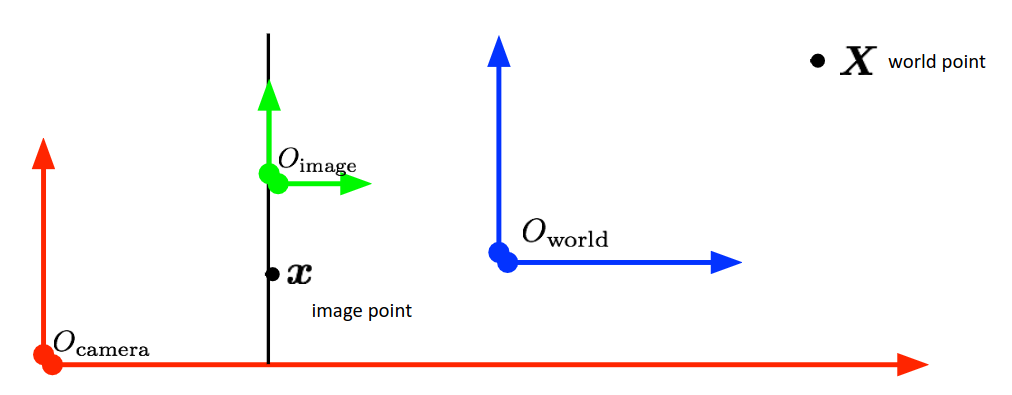
\includegraphics[width=0.75\linewidth]{images/part5/world-to-camera.png}
\end{figure}

\NoteSection{Perspective Projection}

\NoteSubsection{Derivation from similar triangles}

Place the camera center at the origin with the image plane at $z = f$.
A 3-D point in camera coordinates $\widetilde{\mathbf{X}}_c = (X, Y, Z)^\top$
emits a ray through the origin.  That ray intersects the image plane at the
2-D point $(x, y)$.

By similar triangles along both axes:
\[
  \frac{x}{f} = \frac{X}{Z}
  \;\Longrightarrow\; x = \frac{fX}{Z},
  \qquad
  \frac{y}{f} = \frac{Y}{Z}
  \;\Longrightarrow\; y = \frac{fY}{Z}.
\]

This is the \textbf{perspective projection} (also called \emph{central
projection}):
\begin{equation}
  \begin{pmatrix} X \\ Y \\ Z \end{pmatrix}
  \;\longmapsto\;
  \begin{pmatrix} fX/Z \\ fY/Z \end{pmatrix}.
  \label{eq:persp-proj}
\end{equation}

Two key consequences follow immediately:
\begin{itemize}[noitemsep]
  \item \textbf{Depth-dependent scaling:} farther objects appear smaller
        (magnification $m = f/Z$ decreases with $Z$).
  \item \textbf{Nonlinearity:} the division by $Z$ makes perspective projection
        nonlinear in Euclidean coordinates.  Homogeneous coordinates linearize it.
\end{itemize}

\NoteSubsection{Normalized image coordinates ($f=1$)}

Setting $f = 1$ and placing the image plane at $z = 1$ gives the
\emph{normalized} (or \emph{canonical}) projection:
\begin{equation}
  (X, Y, Z)^\top \;\longmapsto\; (X/Z,\; Y/Z)^\top.
  \label{eq:norm-proj}
\end{equation}
These \textbf{normalized image coordinates} $(x_n, y_n) = (X/Z, Y/Z)$ are
independent of any camera-specific parameters and form the intermediate
representation before applying the intrinsic matrix $K$.

\NoteSection{Camera Matrix and Homogeneous Coordinates}

\NoteSubsection{Why homogeneous coordinates?}

As in Part 4, a 2-D point is $(u,v,1)^\top$ up to scale; a 3-D point
likewise becomes $(X,Y,Z,1)^\top$.  The division by $Z$ is then deferred
to a final de-homogenization, making projection \emph{linear}.

\NoteSubsection{Camera as a linear map}

A camera maps homogeneous 3-D world coordinates to homogeneous 2-D image
coordinates:
\begin{equation}
  \mathbf{x} \sim \mathbf{P}\,\mathbf{X}_w,
  \qquad
  \mathbf{x} \in \mathbb{P}^2,\quad \mathbf{X}_w \in \mathbb{P}^3,
\end{equation}
where $\mathbf{P}$ is the $3\times 4$ \textbf{camera matrix} (11 DOF after
removing the overall scale ambiguity from 12 entries).  Expanded:
\[
\begin{pmatrix}
    \tilde{u} \\ \tilde{v} \\ \tilde{w}
\end{pmatrix}
=
\begin{pmatrix}
    p_{11} & p_{12} & p_{13} & p_{14} \\
    p_{21} & p_{22} & p_{23} & p_{24} \\
    p_{31} & p_{32} & p_{33} & p_{34}
\end{pmatrix}
\begin{pmatrix}
    X \\ Y \\ Z \\ 1
\end{pmatrix},
\qquad
(u,v) = \left(\frac{\tilde{u}}{\tilde{w}},\, \frac{\tilde{v}}{\tilde{w}}\right).
\]

\NoteSubsection{Simplest projection matrix ($f=1$, camera at origin)}

When the camera center coincides with the world origin and $f = 1$:
\begin{equation}
  P_0 = \bigl[\,I_{3\times 3} \mid \mathbf{0}\,\bigr]
      = \begin{pmatrix}
          1 & 0 & 0 & 0 \\
          0 & 1 & 0 & 0 \\
          0 & 0 & 1 & 0
        \end{pmatrix}.
\end{equation}
Applying $P_0$ to $(X, Y, Z, 1)^\top$ yields $(X, Y, Z)^\top$ in homogeneous
image coordinates, which de-homogenizes to $(X/Z, Y/Z)^\top$, recovering
the normalized projection~\eqref{eq:norm-proj}.

\NoteSubsection{General focal length $f$}

Scaling the first two rows by $f$ encodes the image-plane distance:
\begin{equation}
  P_f = \begin{pmatrix}
    f & 0 & 0 & 0 \\
    0 & f & 0 & 0 \\
    0 & 0 & 1 & 0
  \end{pmatrix},
  \qquad
  (X,Y,Z,1)^\top \mapsto (fX/Z,\; fY/Z)^\top,
\end{equation}
recovering the full perspective equation~\eqref{eq:persp-proj}.

\NoteSection{Intrinsic Matrix $K$}

The \textbf{intrinsic matrix} $K$ converts normalized image coordinates
$(x_n, y_n)$ to pixel coordinates $(u, v)$.  It bundles all
camera-internal geometric parameters.

\NoteSubsection{Principal-point offset}

The image origin is typically at the sensor corner, not at the principal
point.  Adding offset $(p_x, p_y)$ in pixels:
\begin{equation}
  u = f\,x_n + p_x, \qquad v = f\,y_n + p_y.
\end{equation}
This gives the standard $K$ for a camera with square pixels:
\begin{equation}
  K = \begin{pmatrix}
    f   & 0 & p_x \\
    0   & f & p_y \\
    0   & 0 & 1
  \end{pmatrix}.
\end{equation}
Intrinsic DOF: $f$ (1) $+$ $p_x, p_y$ (2) $=$ 3 intrinsic parameters.
With 6 extrinsic DOF ($\mathbf{R}$: 3, $\mathbf{t}$: 3), the standard
model has $\mathbf{9}$ DOF total.

\NoteSubsection{CCD camera --- non-square pixels}

Digital sensors may have non-square pixels, giving separate effective focal
lengths $f_x$ and $f_y$ (in pixels) along each axis:
\begin{equation}
  K = \begin{pmatrix}
    f_x & 0   & p_x \\
    0   & f_y & p_y \\
    0   & 0   & 1
  \end{pmatrix}, \qquad f_x = f\,s_x,\quad f_y = f\,s_y,
\end{equation}
where $s_x, s_y$ are the pixel densities (pixels per meter).  Adding
$f_y$ as a free parameter brings the intrinsic count to 4, giving
\textbf{10 DOF} total.

\NoteSubsection{Finite projective camera --- sensor skew}

If the pixel axes are not exactly perpendicular (e.g., due to
manufacturing imperfections), a \textbf{skew} parameter $s$ couples the
$x$ and $y$ directions:
\begin{equation}
  K = \begin{pmatrix}
    f_x & s   & p_x \\
    0   & f_y & p_y \\
    0   & 0   & 1
  \end{pmatrix}, \qquad s \neq 0.
\end{equation}
In practice $s \approx 0$ for modern sensors, but the general model with
all 5 intrinsic parameters free gives \textbf{11 DOF} total.  This is the
most general \emph{finite} camera (infinite cameras such as orthographic
are excluded).

\NoteSubsection{Degrees-of-freedom summary}

\begin{center}
\begin{tabular}{lccc}
  \toprule
  Camera model & Intrinsic params & Extra & Total DOF \\
  \midrule
  Standard pinhole        & $f, p_x, p_y$         & ---       & 9  \\
  CCD (non-square pixels) & $f_x, f_y, p_x, p_y$  & $f_y$     & 10 \\
  Finite projective (skew)& $f_x, f_y, s, p_x, p_y$ & $s$    & 11 \\
  \bottomrule
\end{tabular}
\end{center}

\noindent Extrinsic DOF (6) = rotation (3) + translation (3) in all cases.

\NoteSection{Extrinsic Parameters}

\NoteSubsection{World-to-camera coordinate transform}

The \textbf{extrinsic parameters} describe the camera's pose (position and
orientation) in the world.  They transform world coordinates into camera
coordinates before projection.

Let $\widetilde{\mathbf{C}} \in \mathbb{R}^3$ be the camera center's
position in world coordinates, and $\mathbf{R} \in SO(3)$ be the
$3\times 3$ rotation matrix whose columns are the world-frame directions
of the camera's $x$-, $y$-, and $z$-axes.

The world-to-camera transform in Euclidean coordinates is:
\begin{equation}
  \widetilde{\mathbf{X}}_c
  = \mathbf{R}\!\left(\widetilde{\mathbf{X}}_w - \widetilde{\mathbf{C}}\right)
  = \mathbf{R}\,\widetilde{\mathbf{X}}_w \underbrace{- \mathbf{R}\widetilde{\mathbf{C}}}_{\mathbf{t}}.
\end{equation}

\textit{Key insight:} $\mathbf{t} = -\mathbf{R}\widetilde{\mathbf{C}}$
is \emph{not} the camera position but rather the position of the world
origin in camera coordinates.

In homogeneous block form ($4\times 4$), this is an invertible rigid-body
transform:
\begin{equation}
  \mathbf{X}_c
  = \underbrace{\begin{pmatrix} \mathbf{R} & -\mathbf{R}\widetilde{\mathbf{C}} \\
                  \mathbf{0}^\top & 1 \end{pmatrix}}_{[\mathbf{R}\mid\mathbf{t}]_{\text{homog.}}}
    \mathbf{X}_w.
\end{equation}

\NoteSubsection{Recovering the camera center from $\mathbf{t}$}

Given the compact parameterization $P = K[\mathbf{R}\mid\mathbf{t}]$,
the camera center in world coordinates is recovered as:
\begin{equation}
  \widetilde{\mathbf{C}} = -\mathbf{R}^\top\,\mathbf{t}.
\end{equation}

\NoteSection{Full Camera Matrix}

\NoteSubsection{Assembling the pipeline}

The complete projection from world point to pixel is:
\begin{align}
  \mathbf{X}_c &= \bigl[\mathbf{R}\mid\mathbf{t}\bigr]\,\mathbf{X}_w
    & &\text{(extrinsics: world $\to$ camera)} \\
  \mathbf{x}_n &= P_0\,\mathbf{X}_c
    & &\text{(ideal projection with }f=1\text{)} \\
  \mathbf{x}   &= K\,\mathbf{x}_n
    & &\text{(intrinsics: normalized $\to$ pixel).}
\end{align}
Chaining these three steps gives the canonical decomposition of $P$:
\begin{equation}
  \boxed{
    P = K\,\bigl[I \mid \mathbf{0}\bigr]
        \begin{pmatrix} \mathbf{R} & -\mathbf{R}\widetilde{\mathbf{C}} \\
                        \mathbf{0}^\top & 1 \end{pmatrix}
      = K\,[\,\mathbf{R} \mid \mathbf{t}\,],
    \qquad \mathbf{t} = -\mathbf{R}\widetilde{\mathbf{C}}.
  }
\end{equation}

The left $3\times 3$ block of $P$ is $M = K\mathbf{R}$, the product of
an upper-triangular matrix ($K$) and an orthogonal matrix ($\mathbf{R}$).
This structure enables later decomposition via QR.

\NoteSubsection{Block-size summary}

\begin{center}
\begin{tabular}{@{}llll@{}}
  \toprule
  Block & Size & Structure & Physical meaning \\
  \midrule
  $K$           & $3\times 3$ & upper-triangular    & intrinsic camera geometry \\
  $\mathbf{R}$  & $3\times 3$ & orthogonal $SO(3)$  & camera orientation in world \\
  $\mathbf{t}$  & $3\times 1$ & vector              & world origin in camera frame \\
  $P$           & $3\times 4$ & general rank-3      & full projection matrix \\
  \bottomrule
\end{tabular}
\end{center}

\NoteSection{Perspective Distortion}

\NoteSubsection{Depth-dependent magnification}

The image magnification at depth $Z$ is:
\begin{equation}
  m(Z) = \frac{f}{Z}.
\end{equation}
Because $m$ depends on $Z$, objects at different depths are scaled
differently.  This is \textbf{perspective distortion}: parallel lines
converge to \emph{vanishing points}, and depth changes cause apparent
size changes even for rigid objects.

\NoteSubsection{The dolly-zoom (Vertigo) effect}

Doubling $f$ while simultaneously doubling $Z$ keeps the foreground
subject at the same image size ($m = f/Z = \text{const}$), but
background objects --- at a different depth $Z'$ --- are now magnified by
$f'/(Z') = 2f/Z'$, making them appear compressed relative to the
foreground.  This is the basis of the \textbf{dolly-zoom} (``Vertigo
effect'') in cinematography.

\NoteSubsection{Foreshortening and vanishing points}

A set of parallel lines in the world with direction vector $\mathbf{d}$
converges in the image to a single \textbf{vanishing point} at
$\mathbf{v} = K\mathbf{R}\mathbf{d}$ (in homogeneous coordinates).
The horizon line is the set of all vanishing points for horizontal
directions, lying at the image row corresponding to the camera's eye level.

\NoteSection{Alternative Camera Models}

\NoteSubsection{Weak perspective (scaled orthographic)}

When the scene depth variation $\Delta Z$ is small compared to the
average depth $Z_0$ (i.e., $\Delta Z \ll Z_0$), all points are
approximated as being at the same depth $Z_0$.  The depth-dependent
magnification $f/Z$ is then replaced by a single constant scale factor
$m = f/Z_0$:
\begin{equation}
  (X, Y, Z)^\top \;\longmapsto\; (mX,\; mY)^\top,
  \qquad m = \frac{f}{Z_0},
\end{equation}
\begin{equation}
  P_{\text{weak}} =
  \begin{pmatrix}
    m & 0 & 0 & 0 \\
    0 & m & 0 & 0 \\
    0 & 0 & 0 & 1
  \end{pmatrix}.
\end{equation}
This is valid when (1) the scene is very far from the camera, or (2) a
\textbf{telecentric lens} is used (pinhole placed at the front focal
point, admitting only rays parallel to the principal axis).

\NoteSubsection{Orthographic projection}

The special case of weak perspective with $m = 1$ and no origin offset
gives pure \textbf{orthographic projection}: depth is entirely ignored,
and world $x, y$ coordinates map directly to image coordinates.
\begin{equation}
  P_{\text{ortho}} =
  \begin{pmatrix}
    1 & 0 & 0 & 0 \\
    0 & 1 & 0 & 0 \\
    0 & 0 & 0 & 1
  \end{pmatrix}.
\end{equation}
Orthographic projection preserves parallel lines, distances, and ratios
along any direction --- properties lost in perspective projection.
It is accurate for engineering/CAD drawings and telephoto photography of
distant objects.

\NoteSection{Pose Estimation and Camera Calibration}

\textbf{Goal:} Given $N$ point correspondences
$\bigl\{(\mathbf{X}_i,\,\mathbf{x}_i)\bigr\}_{i=1}^{N}$ between known
3-D world points and observed 2-D image points, estimate the $3\times 4$
camera matrix $P$.

\NoteSubsection{Projection equations in inhomogeneous coordinates}

Let $\mathbf{m}_j^\top$ denote the $j$-th row of $P$ (a $1\times 4$
vector).  The projection $\mathbf{x}_i = P\,\mathbf{X}_i$ in homogeneous
form de-homogenizes to:
\begin{equation}
  u_i = \frac{\mathbf{m}_1^\top\,\mathbf{X}_i}{\mathbf{m}_3^\top\,\mathbf{X}_i},
  \qquad
  v_i = \frac{\mathbf{m}_2^\top\,\mathbf{X}_i}{\mathbf{m}_3^\top\,\mathbf{X}_i}.
  \label{eq:proj-het}
\end{equation}
These are rational (nonlinear) functions of $P$'s entries due to the
shared denominator $\mathbf{m}_3^\top\mathbf{X}_i$.

\NoteSubsection{Linearization: Direct Linear Transform (DLT)}

Cross-multiplying~\eqref{eq:proj-het} clears the denominator and yields
two \emph{linear} equations per correspondence:
\begin{align}
  \mathbf{m}_1^\top\,\mathbf{X}_i - u_i\,\mathbf{m}_3^\top\,\mathbf{X}_i &= 0, \\
  \mathbf{m}_2^\top\,\mathbf{X}_i - v_i\,\mathbf{m}_3^\top\,\mathbf{X}_i &= 0.
\end{align}
Stacking these for all $N$ correspondences into a matrix $A \in \mathbb{R}^{2N\times 12}$:
\begin{equation}
  A\,\mathbf{p} = \mathbf{0}, \qquad \mathbf{p} = \operatorname{vec}(P) \in \mathbb{R}^{12}.
\end{equation}
This is a homogeneous linear system: the camera matrix $P$ lies in the
null space of $A$.  Since $P$ has 11 DOF (12 entries, 1 scale), each
correspondence contributes 2 constraints, so $N \geq 6$ correspondences
are needed (actually $N=6$ gives exactly 11 constraints; more gives an
overdetermined system solved in the least-squares sense).

\NoteSubsection{Solution by SVD}

The minimum-norm solution (constrained to $\|\mathbf{p}\|=1$ to avoid
the trivial $\mathbf{p}=\mathbf{0}$) is:
\begin{equation}
  \hat{\mathbf{p}} = \arg\min_{\|\mathbf{p}\|=1} \|A\mathbf{p}\|^2
  = \text{last column of } V \text{ in } A = U\Sigma V^\top.
\end{equation}
Equivalently, $\hat{\mathbf{p}}$ is the eigenvector of $A^\top A$
corresponding to its \emph{smallest} eigenvalue.  This is the
\textbf{DLT algorithm}.

\NoteSection{Camera Matrix Decomposition}

Given an estimated $P$, it is useful to recover the physical parameters
$K$, $\mathbf{R}$, and $\widetilde{\mathbf{C}}$ separately.

\NoteSubsection{Recovering the camera center $\widetilde{\mathbf{C}}$}

By definition, the camera center projects to the zero vector under $P$:
\begin{equation}
  P\,\widetilde{\mathbf{C}}_h = \mathbf{0}
  \;\Longrightarrow\;
  \widetilde{\mathbf{C}}_h = \operatorname{null}(P).
\end{equation}
Numerically, $\widetilde{\mathbf{C}}_h$ is the right singular vector of
$P$ corresponding to the smallest singular value (from $P = U\Sigma V^\top$,
take the last column of $V$).  De-homogenize to get $\widetilde{\mathbf{C}}$.

\NoteSubsection{Recovering intrinsics $K$ and rotation $\mathbf{R}$}

Write $P = [M \mid \mathbf{p}_4]$ where $M = K\mathbf{R}$ is the
left $3\times 3$ block.  Since $K$ is upper-triangular with positive
diagonal and $\mathbf{R}$ is orthogonal, their product $M$ has a unique
factorization via \textbf{RQ decomposition} (a variant of QR):
\begin{equation}
  M = K\mathbf{R}
  \;\xrightarrow{\;\text{RQ}\;}
  K \;\text{(upper-triangular, positive diagonal)},\quad
  \mathbf{R} \;\text{(orthogonal)}.
\end{equation}
Finally, $\mathbf{t} = K^{-1}\mathbf{p}_4$, and the camera center is
$\widetilde{\mathbf{C}} = -\mathbf{R}^\top\mathbf{t}$.

\NoteSection{Nonlinear Refinement and Lens Distortion}

\NoteSubsection{Reprojection error}

The DLT solution minimizes an algebraic error that has no direct geometric
meaning.  The preferred objective is the \textbf{reprojection error} ---
the sum of squared Euclidean distances between observed image points and
their projections under the estimated $P$:
\begin{equation}
  E(K,\mathbf{R},\mathbf{t}) = \sum_{i=1}^{N}
      \left[
        \left(u_i - \frac{\mathbf{m}_1^\top\,\mathbf{X}_i}
                         {\mathbf{m}_3^\top\,\mathbf{X}_i}\right)^{\!2}
        +
        \left(v_i - \frac{\mathbf{m}_2^\top\,\mathbf{X}_i}
                         {\mathbf{m}_3^\top\,\mathbf{X}_i}\right)^{\!2}
      \right].
\end{equation}
Minimized over $K$, $\mathbf{R}$, $\mathbf{t}$ by iterative nonlinear
optimization (typically Levenberg--Marquardt), initialized from the DLT
solution.

\NoteSubsection{Radial lens distortion}

Real lenses deviate from the ideal pinhole model.  The dominant
imperfection is \textbf{radial distortion}: image points are displaced
radially from the principal point.  Let $(x_n, y_n)$ be ideal normalized
coordinates and $r^2 = x_n^2 + y_n^2$.  The distorted normalized coordinates are:

\begin{align}
    x_d &= x_n\,(1 + k_1 r^2 + k_2 r^4 + k_3 r^6 + \cdots),\\
    y_d &= y_n\,(1 + k_1 r^2 + k_2 r^4 + k_3 r^6 + \cdots),
\end{align}

where $k_1, k_2, k_3$ are \textbf{radial distortion coefficients}
estimated during calibration.

\begin{itemize}[noitemsep]
  \item \textbf{Barrel distortion ($k_1 < 0$):} image bulges outward;
        straight lines bow away from center.  Common in wide-angle lenses.
  \item \textbf{Pincushion distortion ($k_1 > 0$):} image pinches inward;
        straight lines bow toward center.  Common in telephoto lenses.
\end{itemize}

The distorted reprojection error adds distortion correction to the pipeline:
$(x_n, y_n) \to (x_d, y_d) \to K \to (u, v)$.

\NoteSection{Calibration Methods}

\NoteSubsection{Reference-object (3-D target) calibration}

Place an object of precisely known 3-D geometry in the scene (e.g., a
calibration rig with marked corner points), identify corresponding 2-D
image points, and solve via DLT.

\begin{itemize}[noitemsep]
  \item \textbf{Pros:} Closed-form solution; straightforward to implement.
  \item \textbf{Cons:} Requires a precisely manufactured 3-D object;
        does not model radial distortion without extension; cannot impose
        known constraints (e.g., known aspect ratio, zero skew).
\end{itemize}

\NoteSubsection{Multi-plane (Zhang's) calibration}

Photograph a flat planar pattern (e.g., checkerboard) from at least 3
different viewpoints.  Corner positions on the plane are known in 2-D
pattern coordinates; their 3-D positions are inferred from the known
planar structure.  Each viewpoint provides a \textbf{homography} (a
$3\times 3$ projective transform between the plane and the image) from
which constraints on $K$ are extracted.
\begin{itemize}[noitemsep]
  \item \textbf{Pros:} Only requires a printed checkerboard; positions
        and orientations of the board need not be known; handles radial
        distortion; implemented in MATLAB (Bouguet toolbox) and OpenCV.
  \item \textbf{Cons:} Requires at least 3 views; involves nonlinear
        optimization for final refinement.
\end{itemize}

\NoteSection{Augmented Reality Application}

The full camera pipeline is illustrated concretely by a simple AR system:
\begin{enumerate}[noitemsep]
  \item \textbf{Detect} known 2-D feature points on a flat AR marker
        (e.g., a QR-code border or checkerboard).
  \item \textbf{Estimate pose} $[\mathbf{R}\mid\mathbf{t}]$ from the
        2-D$\leftrightarrow$3-D correspondences using DLT followed by
        Levenberg--Marquardt refinement on reprojection error.  $K$ is
        pre-calibrated.
  \item \textbf{Render virtual content} by projecting 3-D virtual geometry
        through the estimated $P = K[\mathbf{R}\mid\mathbf{t}]$:
        \[
          \mathbf{x}_{\text{virtual}} \sim P\,\mathbf{X}_{\text{3D}}.
        \]
  \item \textbf{Composite} the rendered virtual image onto the live camera
        feed, producing the AR output.
\end{enumerate}
The quality of the overlay depends directly on the accuracy of $K$
(calibration) and $[\mathbf{R}\mid\mathbf{t}]$ (pose estimation).





\end{notes}
\end{document}
